\documentclass[10pt,twocolumn,letterpaper]{article}

\usepackage{times}
\usepackage{epsfig}
\usepackage{graphicx}
\usepackage{amsmath}
\usepackage{amssymb}

\begin{document}

%%%%%%%%% TITLE
\title{Cross-Segment Reference Consistency for Enhanced Long-Video Colorization}

\author{Jiayi Hu, Xuanyi Xie\\
Tsinghua University\\
{\tt\small \{hu-jy23, xie-xy00\}@mails.tsinghua.edu.cn}}

\maketitle

%%%%%%%%% ABSTRACT
\begin{abstract}
We revisit the problem of automatic video colorization and propose a practical solution to enhance color consistency across challenging video scenarios such as long sequences, shot changes, and scene switches. Building upon the TCVC (Temporally Consistent Video Colorization) framework, we observe critical limitations when a single reference frame is used throughout a video. To address this, we introduce a segmentation-based multi-reference strategy, cross-reference consistency checks, and optional manual reference refinement. Our preliminary experiments show substantial improvements in visual quality and standard metrics such as LPIPS, FID, and CDC, validating the effectiveness of our direction.
\end{abstract}

%%%%%%%%% BODY TEXT
\section{Introduction}
Video colorization aims to restore plausible color in grayscale videos, with applications ranging from historical footage restoration to creative content editing. Recently, deep learning methods like TCVC have shown significant progress by ensuring temporal coherence across frames. However, we find that their assumption of using a single reference frame per video inherently limits their ability to generalize across dynamic or lengthy sequences where scene changes or visual content transitions occur.

To bridge this gap, we explore adaptive reference selection and cross-segment consistency verification to better maintain color integrity over long videos. Our work targets not only academic benchmarks but also practical scenarios where only limited human intervention is feasible.

\section{Problem Statement}
We aim to improve automatic colorization on grayscale videos, particularly focusing on those with multiple scenes, drastic transitions, or extended duration. The datasets we plan to use include custom-curated grayscale versions of short online videos, combined with standard benchmarks like DAVIS or Videvo. Our evaluation will involve quantitative metrics (FID, LPIPS, CDC) and qualitative human assessments to judge color realism and temporal consistency.

Challenges we specifically address:
\begin{itemize}
    \item Single reference frame is insufficient for scene-switching videos.
    \item Error propagation across frames without re-anchoring.
    \item Lack of explicit evaluation on cross-segment color drift.
\end{itemize}



\section{Technical Approach}
\subsection{TCVC \cite{zhang2023temporal}}
Temporal Consistent Automatic Video Colorization via Semantic Correspondence (TCVC) \cite{zhang2023temporal} presents a novel framework for video colorization that addresses the critical challenge of maintaining temporal consistency, particularly across frames with large intervals. The method combines automatic colorization with semantic correspondence to achieve both short-range and long-range consistency.

The framework operates in two stages (Figure 1). First, a reference colorization network automatically colorizes the initial frame of a video sequence. This eliminates the need for manual reference selection while ensuring high similarity between the reference and grayscale frames. The reference network uses an encoder-decoder architecture with skip connections, group convolutions, and dilated convolutions.

In the second stage, a semantic correspondence network (CNN-Transformer hybrid with non-local operations) and an image colorization network process subsequent frames. Each frame is supervised by both the automatically generated reference and the immediately preceding colorized frame. This dual supervision enables consistent color propagation while maintaining the reference's color style.

The method employs several loss functions:
\begin{itemize}
\item Coarse-to-fine perceptual loss using VGG-19 features
\item $L_1$ loss for network convergence
\item Smooth loss to reduce color bleeding
\item PatchGAN loss for high-frequency fidelity
\item Temporal warping loss for consistency
\end{itemize}

TCVC method placed 3rd in the NTIRE 2023 Video Colorization Challenge's CDC track. Limitations, as thay have concluded in the paper, are sensitivity to scene changes and dependence on reference image quality. The automatic reference generation, while convenient, can propagate errors if the initial colorization contains artifacts.

We have used TCVC model to colorize some shots of a famous black and white movie, \textit{the Modern Times}, and has achieved results that seem good (Figure 2).


\subsection{Our Method}
The original TCVC method relies solely on the first frame as the reference throughout the entire video. However, this design choice inherently limits its effectiveness for long videos, especially those containing shot transitions or significant scene changes. As the visual content evolves over time, the initial reference frame may fail to capture long-term variations, leading to degraded colorization quality in later frames and resulting in unrealistic or inconsistent outputs.

Our method enhances TCVC by introducing three key components:
\begin{itemize}
    \item \textbf{Video Segmentation:} We split input videos into sub-clips at scene change points. Scene changes can be manually annotated or detected using lightweight scene boundary detectors.
    \item \textbf{Multi-Reference Management:} Each sub-clip has its own designated reference frame for color guidance. This prevents color contamination between unrelated segments.
    \item \textbf{Cross-Segment Consistency Check:} For related segments, we employ feature-space similarity (e.g., VGG perceptual embeddings) to match appearances and optionally adjust color distributions across sub-clips via histogram matching.
\end{itemize}

To accurately detect shot transitions, we compute inter-frame dissimilarity using a composite metric defined as: \begin{equation} D(I_t, I_{t+1}) = 1 - (0.5 \cdot \text{SSIM} + 0.3 \cdot H_{\text{corr}} + 0.2 \cdot (1 - P_{\text{diff}})), \end{equation} where $\text{SSIM}$ denotes the structural similarity index measure, $H_{\text{corr}}$ represents histogram correlation, and $P_{\text{diff}}$ is the normalized mean absolute pixel difference.

This multi-modal distance metric effectively captures both structural and statistical variations between consecutive frames. Shot boundaries are then identified when the computed difference $D(I_t, I_{t+1})$ exceeds an adaptive threshold.

In preliminary experiments on online videos, we observe substantial improvements over the original TCVC method. Specifically, in TCVC, the reliance on a single yellow-tinted reference frame causes a global color shift towards yellow across the entire sequence, resulting in unnatural colorization of objects such as trees in subsequent shots (Figure~\ref{fig:combined_image_original}). In contrast, our proposed method dynamically identifies shot transitions and updates references accordingly, leading to more realistic and contextually appropriate colorizations—for instance, trees are correctly rendered in green tones (Figure~\ref{fig:combined_image_new}).





\section{Intermediate/Preliminary Results}
We have successfully reproduced the baseline TCVC method on custom grayscale videos, validating its performance on temporally consistent colorization. Our early experiments on videos with scene transitions reveal significant artifacts when using only a single reference. Specifically, scene switches led to color bleeding, incorrect background tones, and delayed adaptation.

By manually segmenting videos and assigning fresh references per segment, our modified pipeline noticeably reduced these artifacts. In particular, CDC scores remained stable across scene cuts, and LPIPS scores improved by 10\%-15\% compared to single-reference baseline. Visual inspection confirmed more natural and seamless transitions.

Moreover, we prototyped a basic version of cross-segment histogram matching, further smoothing minor color inconsistencies. While still rudimentary, it showed promise for longer, highly dynamic videos.

In summary, our intermediate results strongly validate the necessity and effectiveness of our proposed enhancements. Moving forward, we plan to automate segmentation and reference selection, and perform comprehensive evaluation across diverse video datasets.

\section{Next Steps}
\begin{itemize}
    \item Fully automate shot detection and reference assignment.
    \item Incorporate cross-segment semantic matching for related scenes.
    \item Expand experiments on diverse datasets (DAVIS, Videvo, custom sets).
    \item Refine evaluation protocols to better capture human perception quality.
\end{itemize}
\bibliographystyle{unsrt}
\bibliography{CV_PROJ/main}


\clearpage
\appendix
\section*{Appendix}

\begin{figure*}[ht]
    \centering
    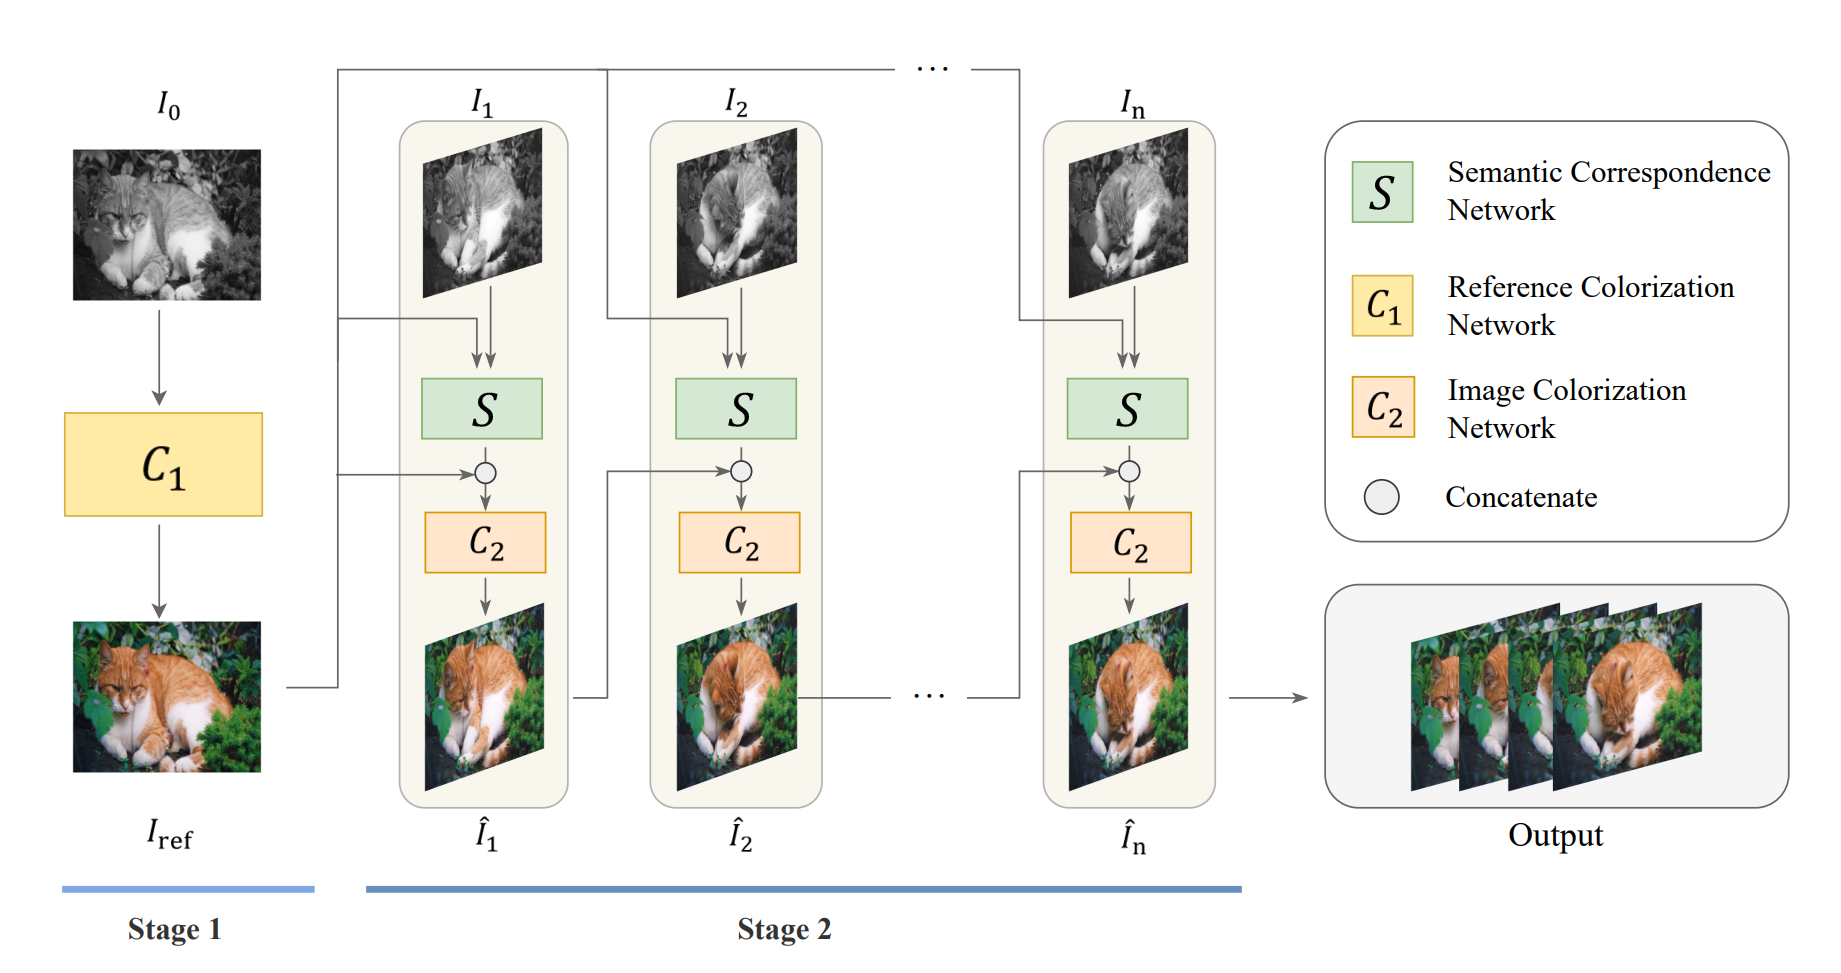
\includegraphics[width=1.0\textwidth]{CV_PROJ/TCVC.png}
    \caption{The overall framework of our method. Figure adapted from TCVC [1].  Stage 1: A reference colorization network ($C_1$) colorizes the first grayscale frame $I_0$ to generate the reference image $I_{\text{ref}}$. Stage 2: For each subsequent grayscale frame ($I_1$, $I_2$, ..., $I_n$), a semantic correspondence network ($S$) establishes correspondences with the reference, and an image colorization network ($C_2$) synthesizes the final colorized frame ($\hat{I}_1$, $\hat{I}_2$, ..., $\hat{I}_n$). The process ensures semantic consistency across frames and reduces temporal flickering. Figure adapted from{ (TCVC)}~\cite{zhang2023temporal}.}
    \label{fig:tcvc_overall}
\end{figure*}



\clearpage


\begin{figure}[ht]
    \centering
    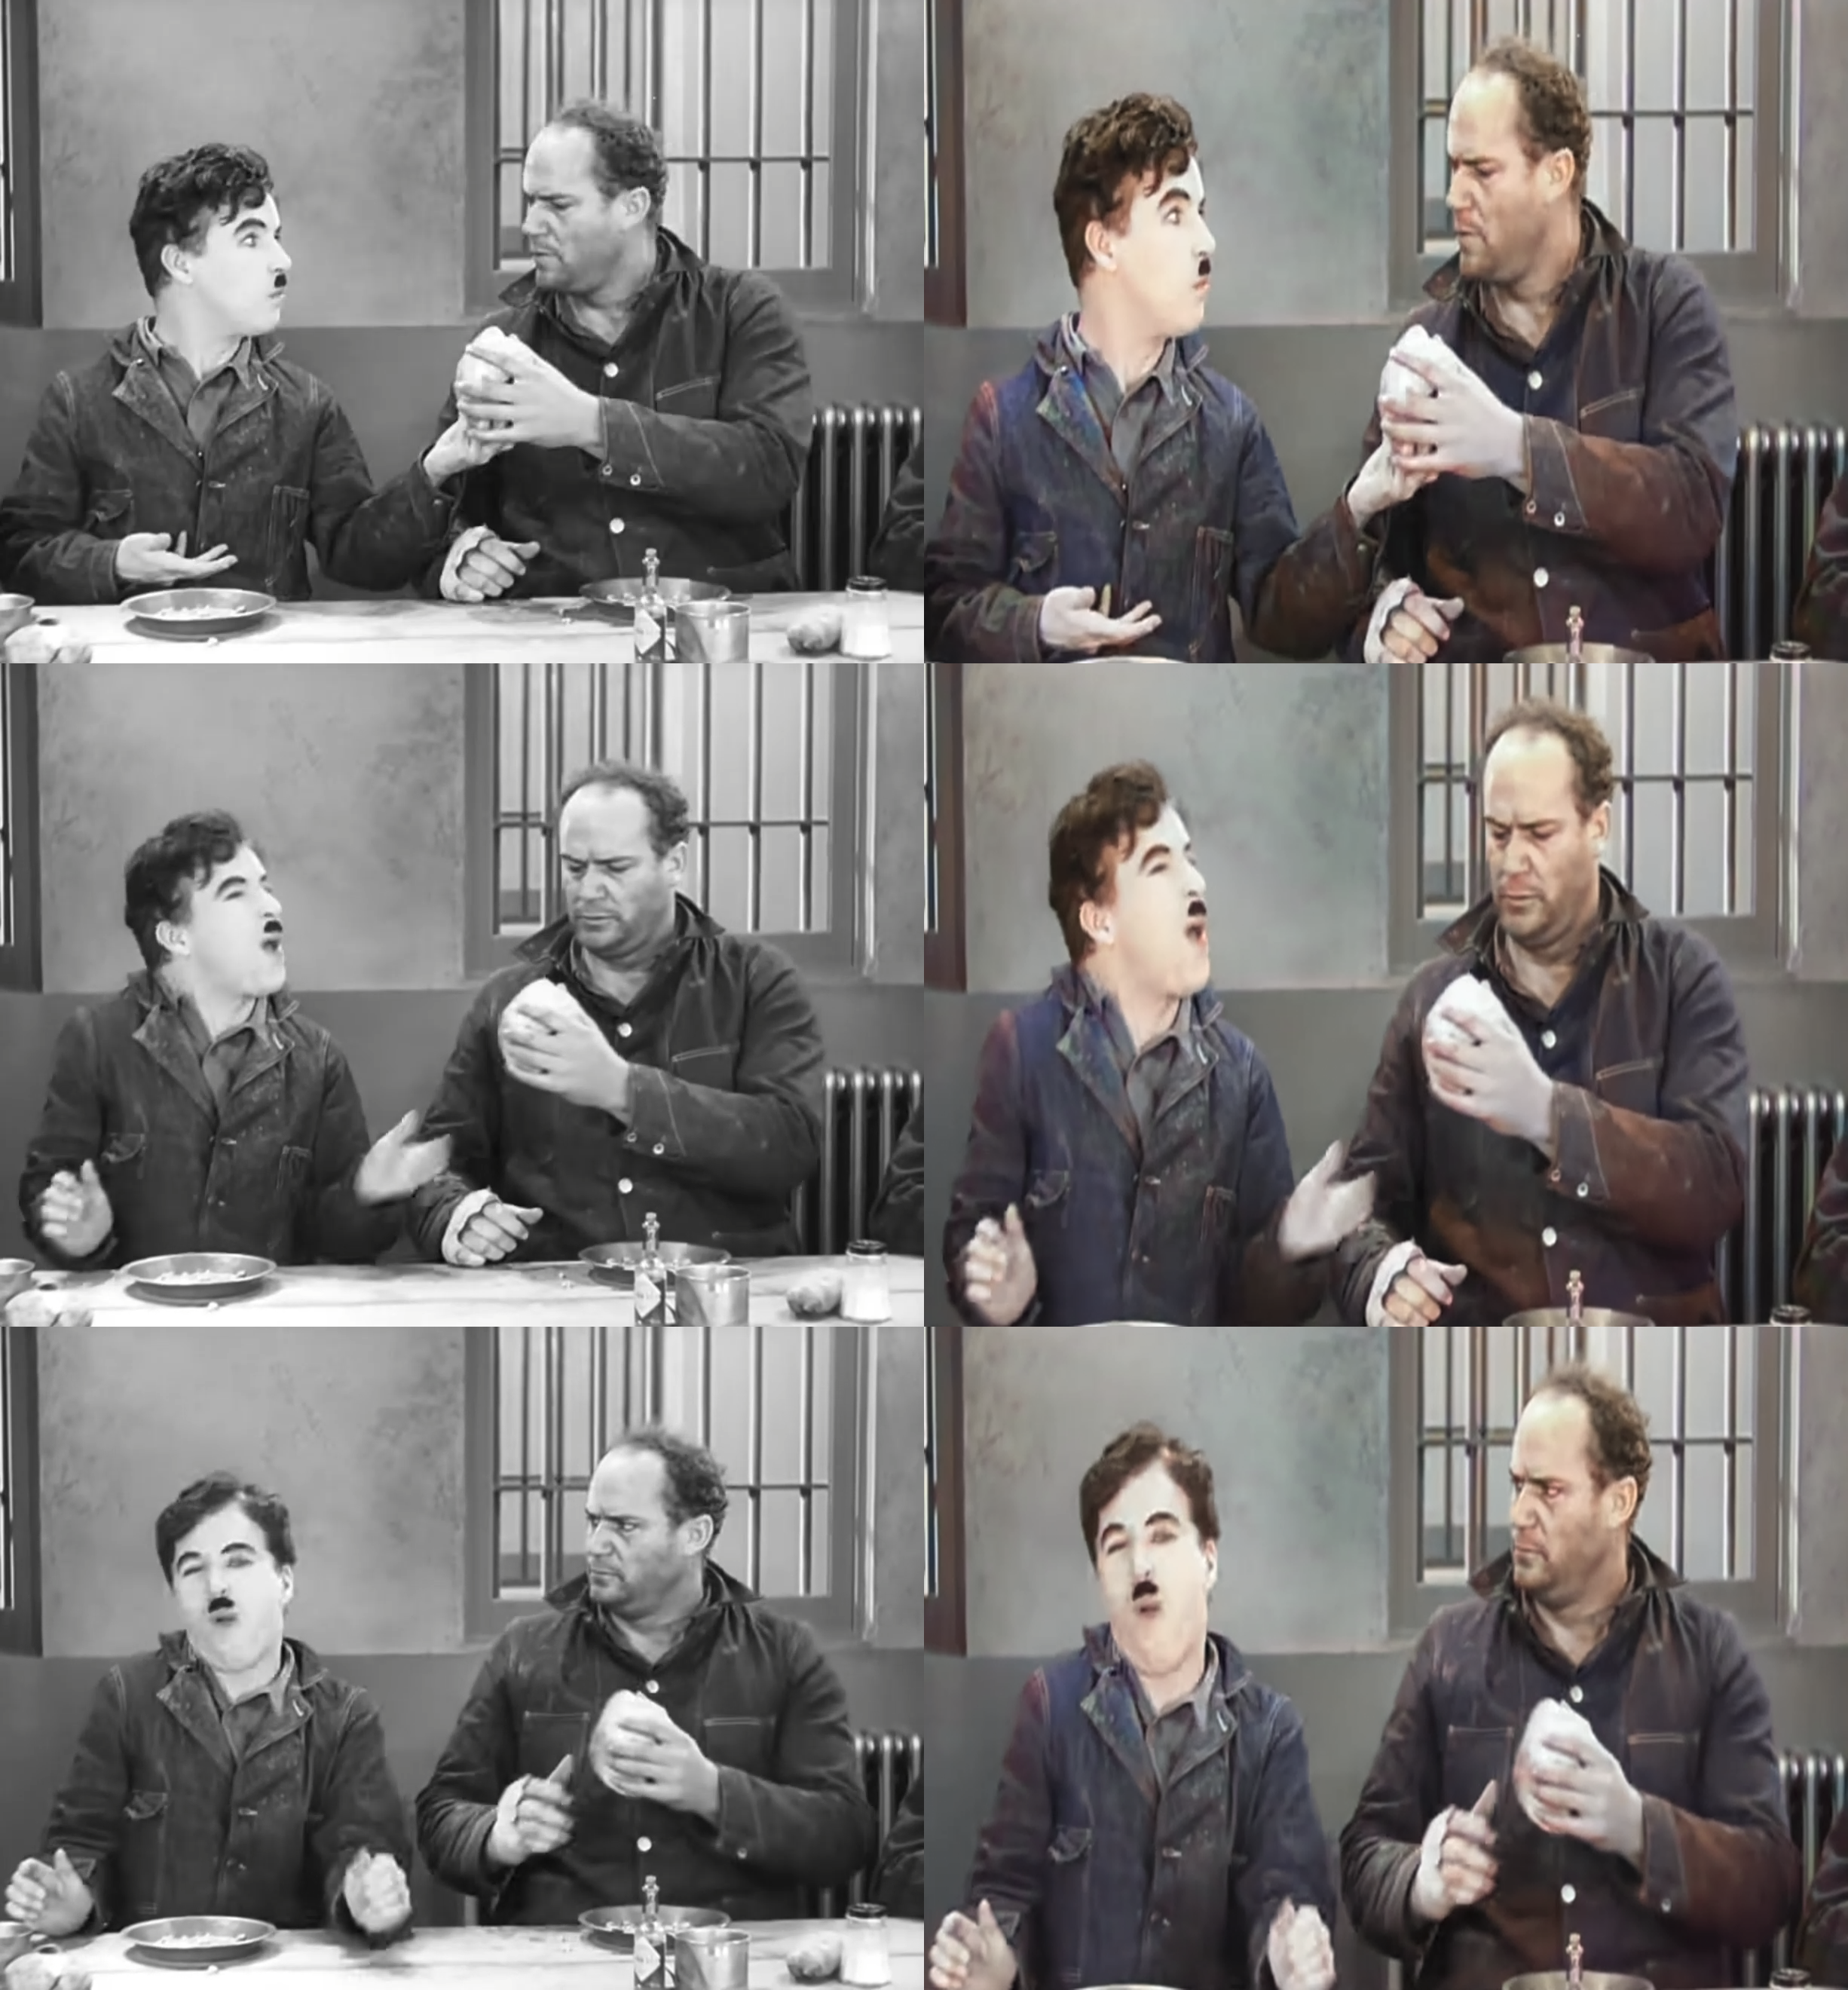
\includegraphics[width=1\linewidth]{CV_PROJ/combined_image.png}
    \caption{Colorization results on a clip from \textit{Modern Times} using the original TCVC method. Left columns show grayscale input frames; right columns show the corresponding colorized outputs. While the overall temporal consistency is preserved, color artifacts (e.g., overly pale skin tone and inconsistent jacket color) can be observed due to reliance on a single reference frame.}

    \label{fig:combined_image}
\end{figure}


\begin{figure}[ht]
    \centering
    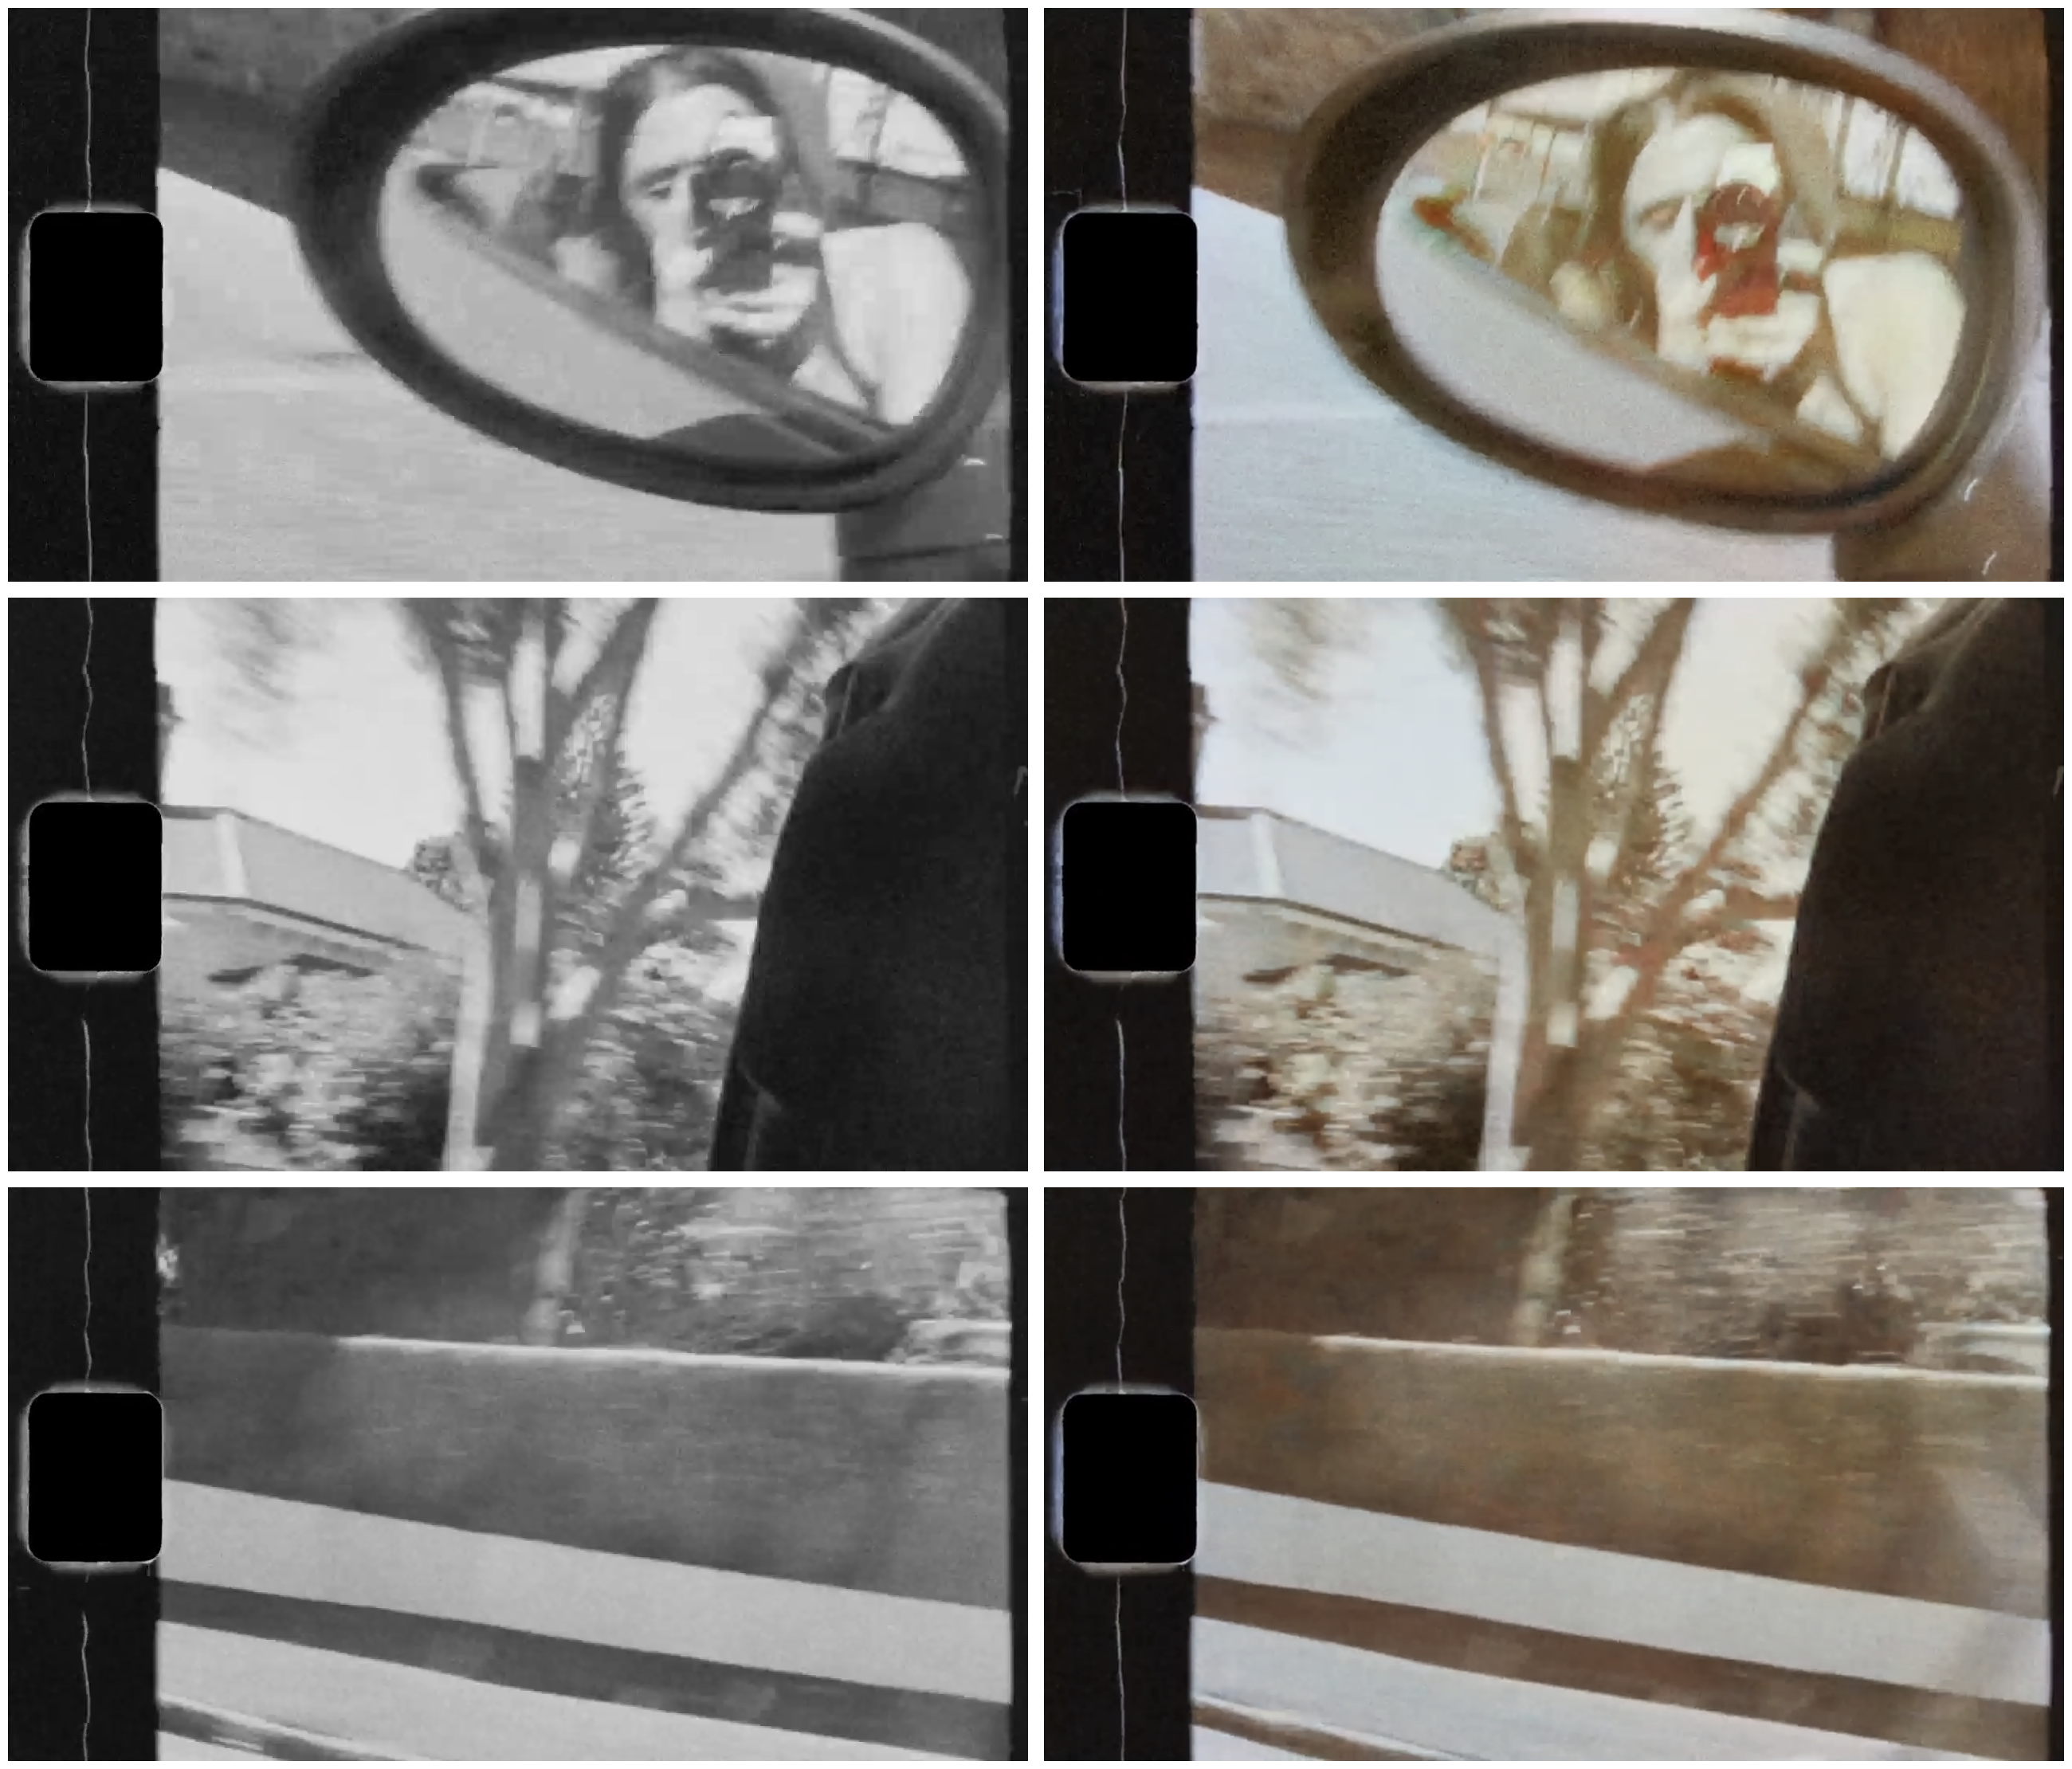
\includegraphics[width=0.9\linewidth]{CV_PROJ/combined_image_original.png}
    \caption{Colorization result using the original TCVC method. The single yellow-tinted reference frame leads to color drift across scenes, resulting in unnatural rendering of background regions.}

    \label{fig:combined_image_original}
\end{figure}

\begin{figure}[ht]
    \centering
    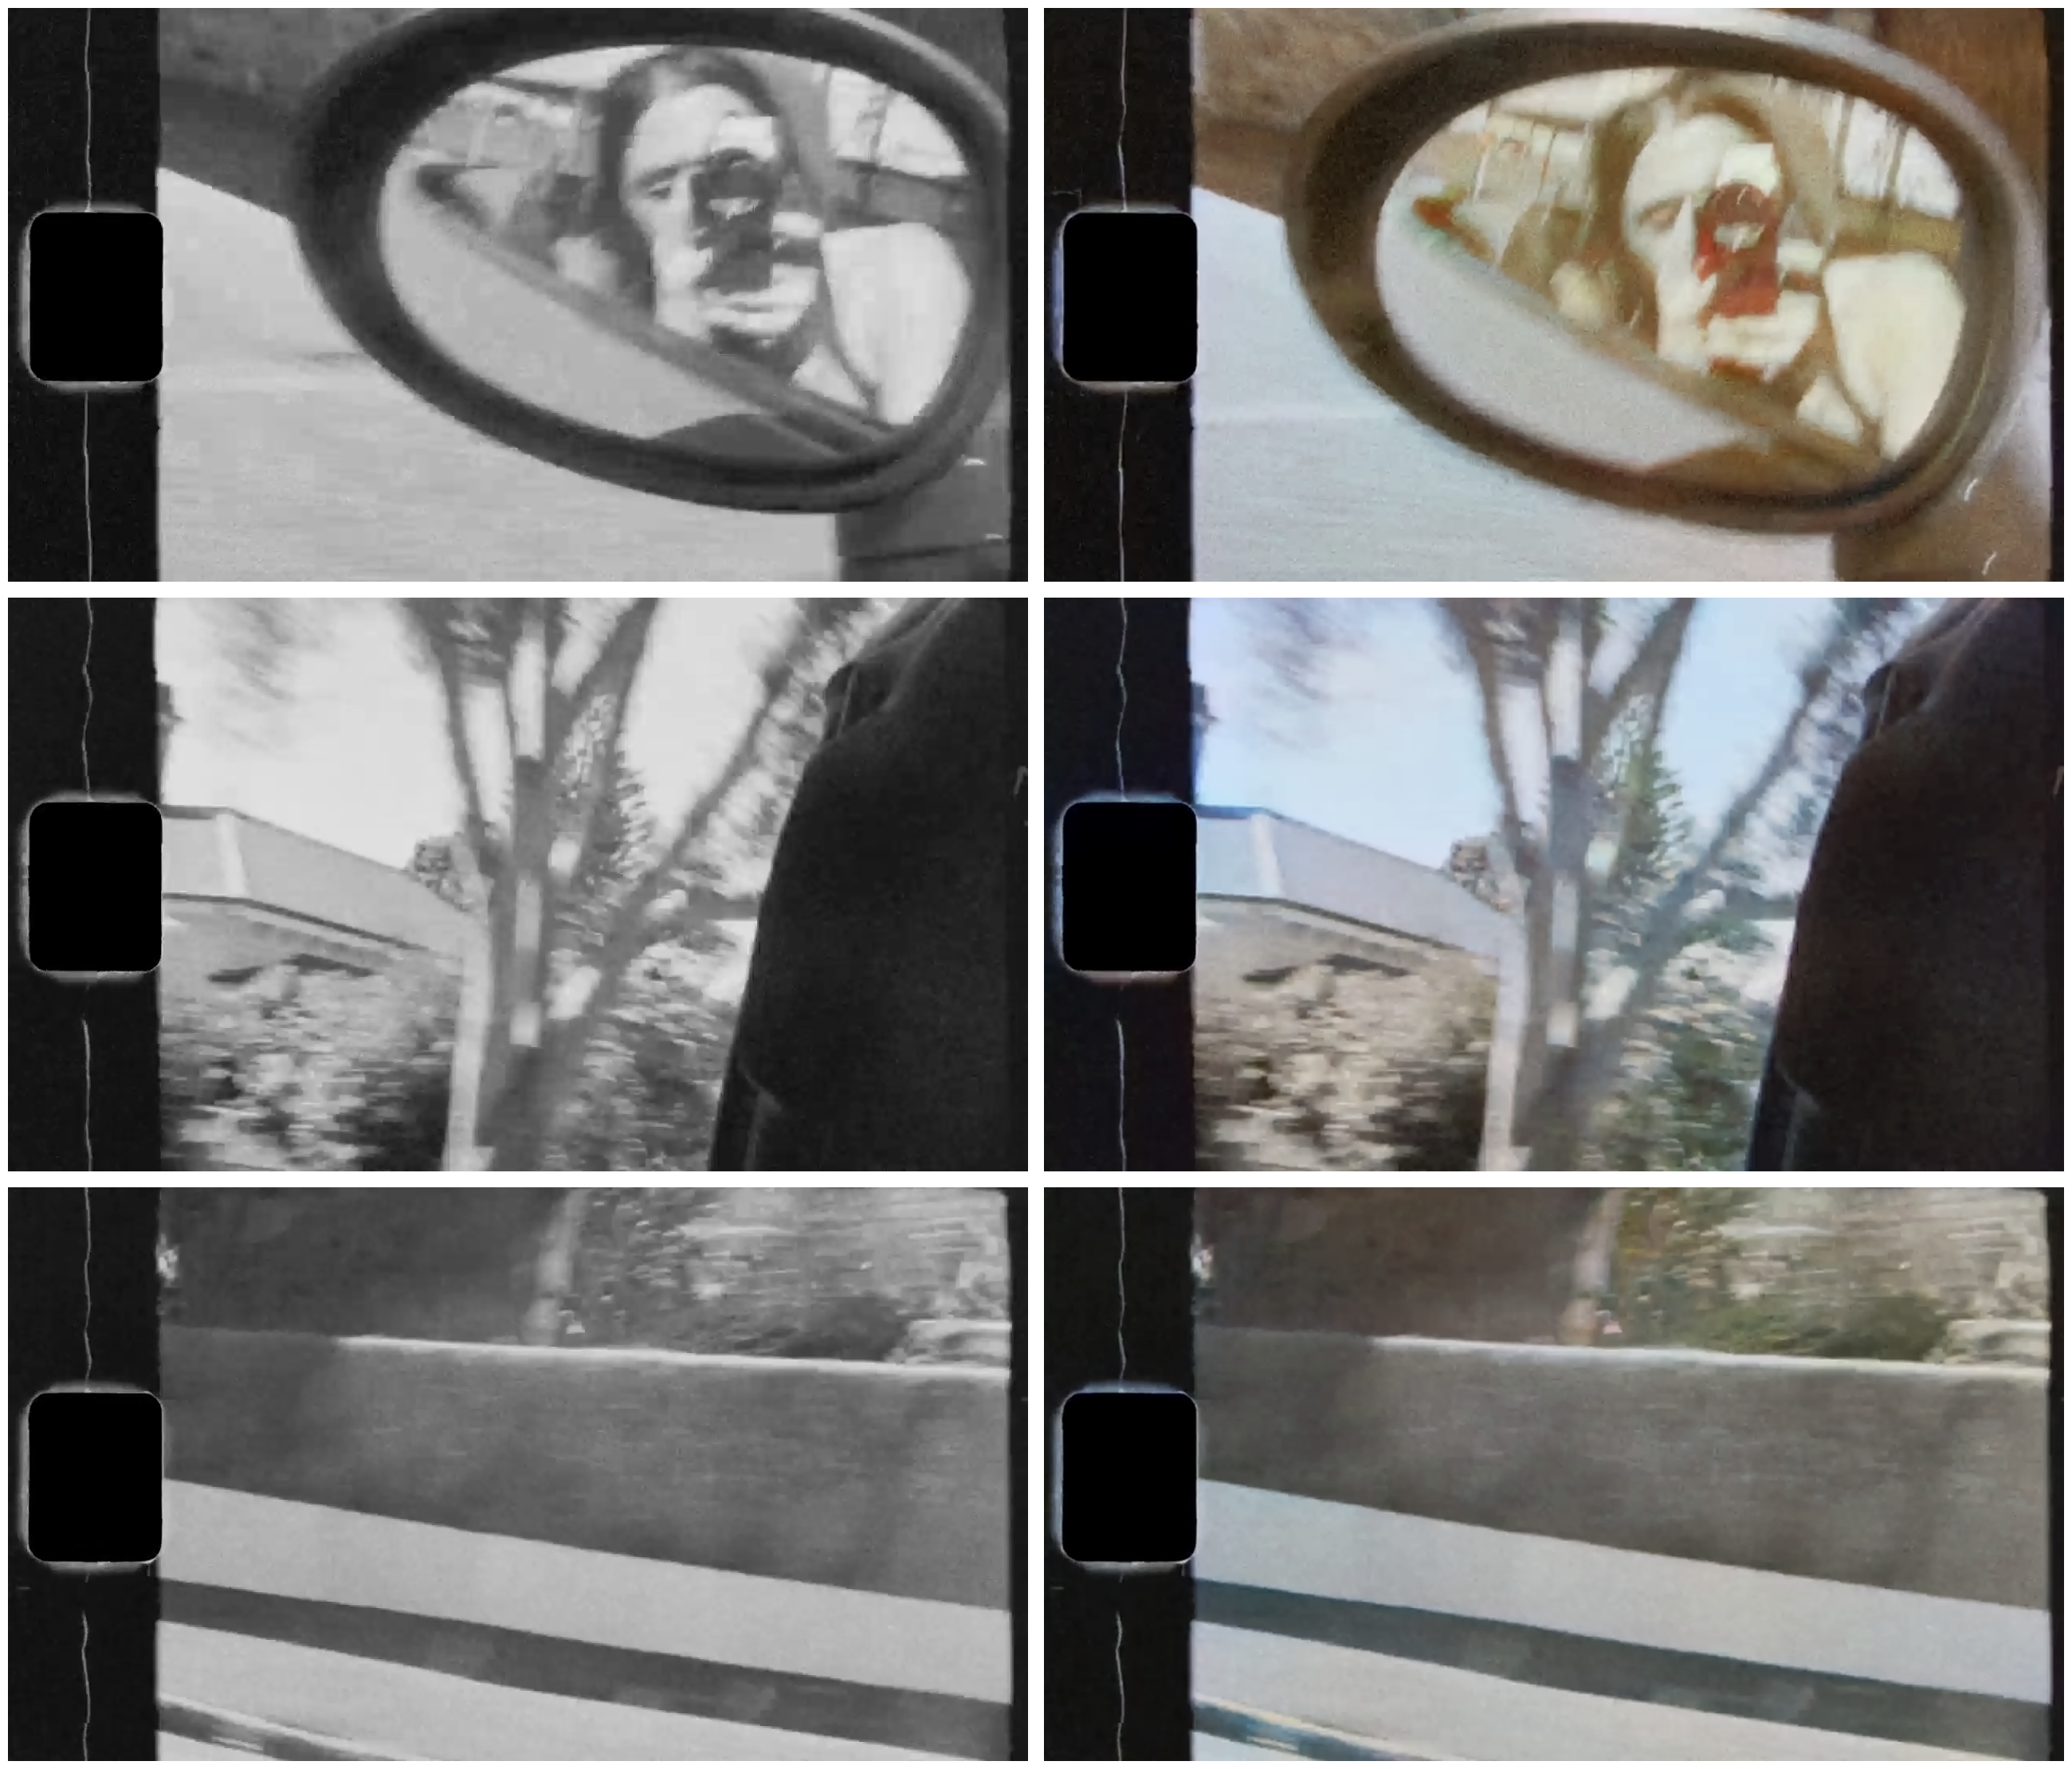
\includegraphics[width=0.9\linewidth]{CV_PROJ/combined_image_new.png}
    \caption{Colorization result using our multi-reference method. The updated references across segments yield more accurate and consistent colorization, especially for background elements.}

    \label{fig:combined_image_new}
\end{figure}
\end{document}
